\chapter{Implementation}

% \documentclass[12pt]{article}

% \usepackage[utf8]{inputenc}
% \usepackage[T1]{fontenc}
% \usepackage{lmodern}        % For improved text clarity
% \usepackage{geometry}       % For page layout
% \usepackage{hyperref}       % For hyperlinks
% \usepackage{graphicx}       % For figures/images
% \usepackage{listings}       % For code listings
% \usepackage{amsmath,amssymb}

% % Set up the listings environment for Python

% \begin{document}

% \section{Implementation}

\section{Pipeline}

The pipeline is implemented through four Jupyter notebooks, one for each module.

\subsection{Template image selection module}

The template image selection module contains an adapter function that reads images from the public LARD dataset \cite{ducoffe_lard_2023}, generates JSON label files, and places the image-label file pairs into the output directory. 
The LARD dataset is composed of several different folders containing both synthetic and real images. 
It has two real images folders: \emph{Nominal cases} and \emph{Edge cases}, the latter being composed of images with poor runway visibility.

Because the template images are used to extract canny edges, it is better to use images with clear runway and surrounding area visibility. 
Hence, the \emph{Nominal cases} folder, containing 1500 images, was chosen.

The images are then processed into square format, since Stable Diffusion naturally works with square images. 
The runway is horizontally centered so it will not be out of frame when cropping into a square. 
The following code does this:

\begin{lstlisting}
xs = [p[0] for p in pts]
ys = [p[1] for p in pts]
min_x, max_x = min(xs), max(xs)
min_y, max_y = min(ys), max(ys)

# Vertical crop is the entire height
top = 0
bottom = H

# Horizontal positioning for H-wide crop
center_x = (min_x + max_x) / 2.0
ideal_left = int(round(center_x - (H / 2)))
left = max(0, min(ideal_left, W - H))
right = left + H

cropped_img = img.crop((left, top, right, bottom))
\end{lstlisting}

Then, the new shifted runway corners' keypoints are computed to build a JSON label:

\begin{lstlisting}
shifted_pts = [(p[0] - left, p[1] - top) for p in pts]

# Build label
image_label = ImageLabel(
    dataset="LARD/LARD_test_real_nominal",
    sourceImage=os.path.basename(image_path),
    runwayLabel=shifted_pts
)
\end{lstlisting}

Finally, the image label is converted to JSON, and both the cropped images and their labels are saved to the output folder.

\subsection{Edge extraction module}

The edge extraction module contains a generator function that takes an input directory and outputs a directory with corresponding canny edge images at a $1024 \times 1024$ resolution. 
The generator function uses an image processor from a ControlNet Auxiliary library to generate the canny edges, and then resizes to the desired resolution:

\begin{lstlisting}
from controlnet_aux.processor import Processor

processor = Processor(
    'canny',
    {
        "detect_resolution": 756,
        "image_resolution": 1024
    }
)

pil_in = Image.open(image_path).convert("RGB")
canny_pil = processor(pil_in, to_pil=True).resize((1024, 1024))
\end{lstlisting}

To help in the image generation process, a polygon is drawn onto the image to delimit the area of the runway:

\begin{lstlisting}
cv2.polylines(
    canny_array,
    [corners_sorted.astype(np.int32)],
    isClosed=True,
    color=(255, 255, 255),
    thickness=2
)
\end{lstlisting}

Finally, the corners are scaled to this new image resolution and saved to the new label file:

\begin{lstlisting}
orig_h, orig_w = image_bgr.shape[:2]
corners_array = np.array(runway_corners, dtype=np.float32)
corners_array[:, 0] *= (1024.0 / orig_w)
corners_array[:, 1] *= (1024.0 / orig_h)
\end{lstlisting}

\subsection{Base Image generation module}

This is the most important module of the pipeline, as everything depends on the quality of the base images generated in this step. 
To generate the images, the \texttt{diffusers} library \cite{???} is used, providing utilities for generating images with diffusion models.

The classes one needs from \texttt{diffusers} depend on which model is in use. 
The DreamShaper model \cite{???} is a general-purpose Stable Diffusion model, meant to compete with other general-purpose models such as DALL-E and Midjourney. 
Of several tested models and pipelines, DreamShaper was chosen for its image quality, faithfulness to the prompt, and ability to construct diverse scenarios (ranging across different lighting and weather conditions).

From the DreamShaper family, we chose the DreamShaper XL version, capable of producing $1024 \times 1024$ images, as it is based on Stable Diffusion XL. 
This higher resolution was necessary to generate finer details such as runway markings.

Having selected DreamShaper XL, the rest follows naturally. 
For the ControlNet model, the pre-trained canny-edge-based ControlNet offered by \texttt{diffusers} for Stable Diffusion XL was used, and the recommended scheduler configuration for DreamShaper was applied:

\begin{lstlisting}
controlnet = ControlNetModel.from_pretrained(
    "diffusers/controlnet-canny-sdxl-1.0", torch_dtype=torch.float16
)

pipeline = StableDiffusionXLControlNetPipeline.from_pretrained(
    "lykon/dreamshaper-xl-v2-turbo",
    torch_dtype=torch.float16,
    variant="fp16",
    controlnet=controlnet
).to("cuda")

pipeline.scheduler = DPMSolverMultistepScheduler.from_config(
    pipeline.scheduler.config,
    algorithm_type="sde-dpmsolver++",
    use_karras_sigmas=True
)

pipeline.enable_model_cpu_offload()
\end{lstlisting}

A critical part of generative models is \emph{prompt engineering}: crafting an input prompt that achieves the desired result. 
Diffusion models accept both a \emph{prompt} and a \emph{negative prompt}. 
The model tries to produce what is mentioned in the prompt and avoid what is mentioned in the negative prompt.

Crafting the prompt is a process of trial and error until satisfactory results are found. 
In practice, it is helpful to look at prompts used in the model's example pages to see keywords the model responds strongly to, such as \texttt{cinematic film still}, \texttt{realistic}, \texttt{ugly}, or \texttt{deformed}.

Since this project needed to create images under diverse scenarios, two base prompts were defined for daylight images with no weather adversity, and a dictionary of modifiers was used to add or remove keywords to achieve weather or time-of-day effects:

\begin{lstlisting}
base_prompt = "photo of airport runway, aerial view, 4k, cinematic film still, realistic, beautiful landscape around, high-contrast runway lines"

base_neg = "airplane, ugly, low-quality, ugly background, ugly airstrip, deformed, dark, noisy, blurry, low contrast, missing lines, unrealistic, drawing, objects on runway"

modifiers = {
    "rain": (
        "+raining +storm +wet",
        "-dark -noisy -blurry",
    ),
    "fog": (
        "+(harsh fog) +mist +haze",
        "-dark -noisy -blurry",
    ),
    "snow": (
        "+snowing",
        "",
    ),
    "dusk": (
        "+(at dusk)",
        "",
    ),
    "dawn": (
        "+(at dawn)",
        "",
    ),
    "night": (
        "+(at night)",
        "-dark",
    )
}
\end{lstlisting}

A helper function (e.g., \texttt{apply\_modifiers}) builds the final prompts (and negative prompts) from the base prompts and these modifiers. 
It also receives the number of images to generate, returning a data structure that can be passed to \texttt{generate\_base\_images}, which uses the prompt pairs to generate and save images:

\begin{lstlisting}
generate_base_images(
    "p_FilteredCannyEdges",  # input directory
    "p_BaseImages",          # output directory
    prompt_pairs=[           # images to generate
        apply_modifiers("day", [], 5),
        apply_modifiers("night", ["night"], 5),
        apply_modifiers("dusk", ["dusk"], 1),
        apply_modifiers("dawn", ["dawn"], 1),
        apply_modifiers("fog", ["fog"], 1),
        apply_modifiers("fog+night", ["night", "fog"], 1),
        apply_modifiers("rain", ["rain"], 1),
        apply_modifiers("rain+night", ["night", "rain"], 1),
        apply_modifiers("snow", ["snow"], 1),
        apply_modifiers("snow+night", ["night", "snow"], 1),
    ],
    model_name="sdxl-dreamshaperxl",
    # show=True
)
\end{lstlisting}

\subsection{Variant image generation module}

To generate variant images, three pipelines are run: a positional variant augmentation, outpainting the borders, and weather occlusion effects.

The first pipeline uses the \emph{Albumentations} library \cite{???} to run three transformations: 
(1) random horizontal flip, 
(2) padding with a border (to simulate a more distant runway), and 
(3) slight random rotation from $-25^\circ$ to $+25^\circ$:

\begin{lstlisting}
pipeline = A.ReplayCompose(
    [
        A.HorizontalFlip(p=0.5),
        A.CropAndPad(
            px=((51, 410),  # top
                (51, 410),  # bottom
                (51, 410),  # left
                (51, 410)), # right
            keep_size=False,
            p=1.0
        ),
        A.Affine(rotate=(-25, 25), p=1.0),
    ],
    keypoint_params=A.KeypointParams(format='xy', remove_invisible=False)
)
\end{lstlisting}

\begin{figure}[htbp]
\centering
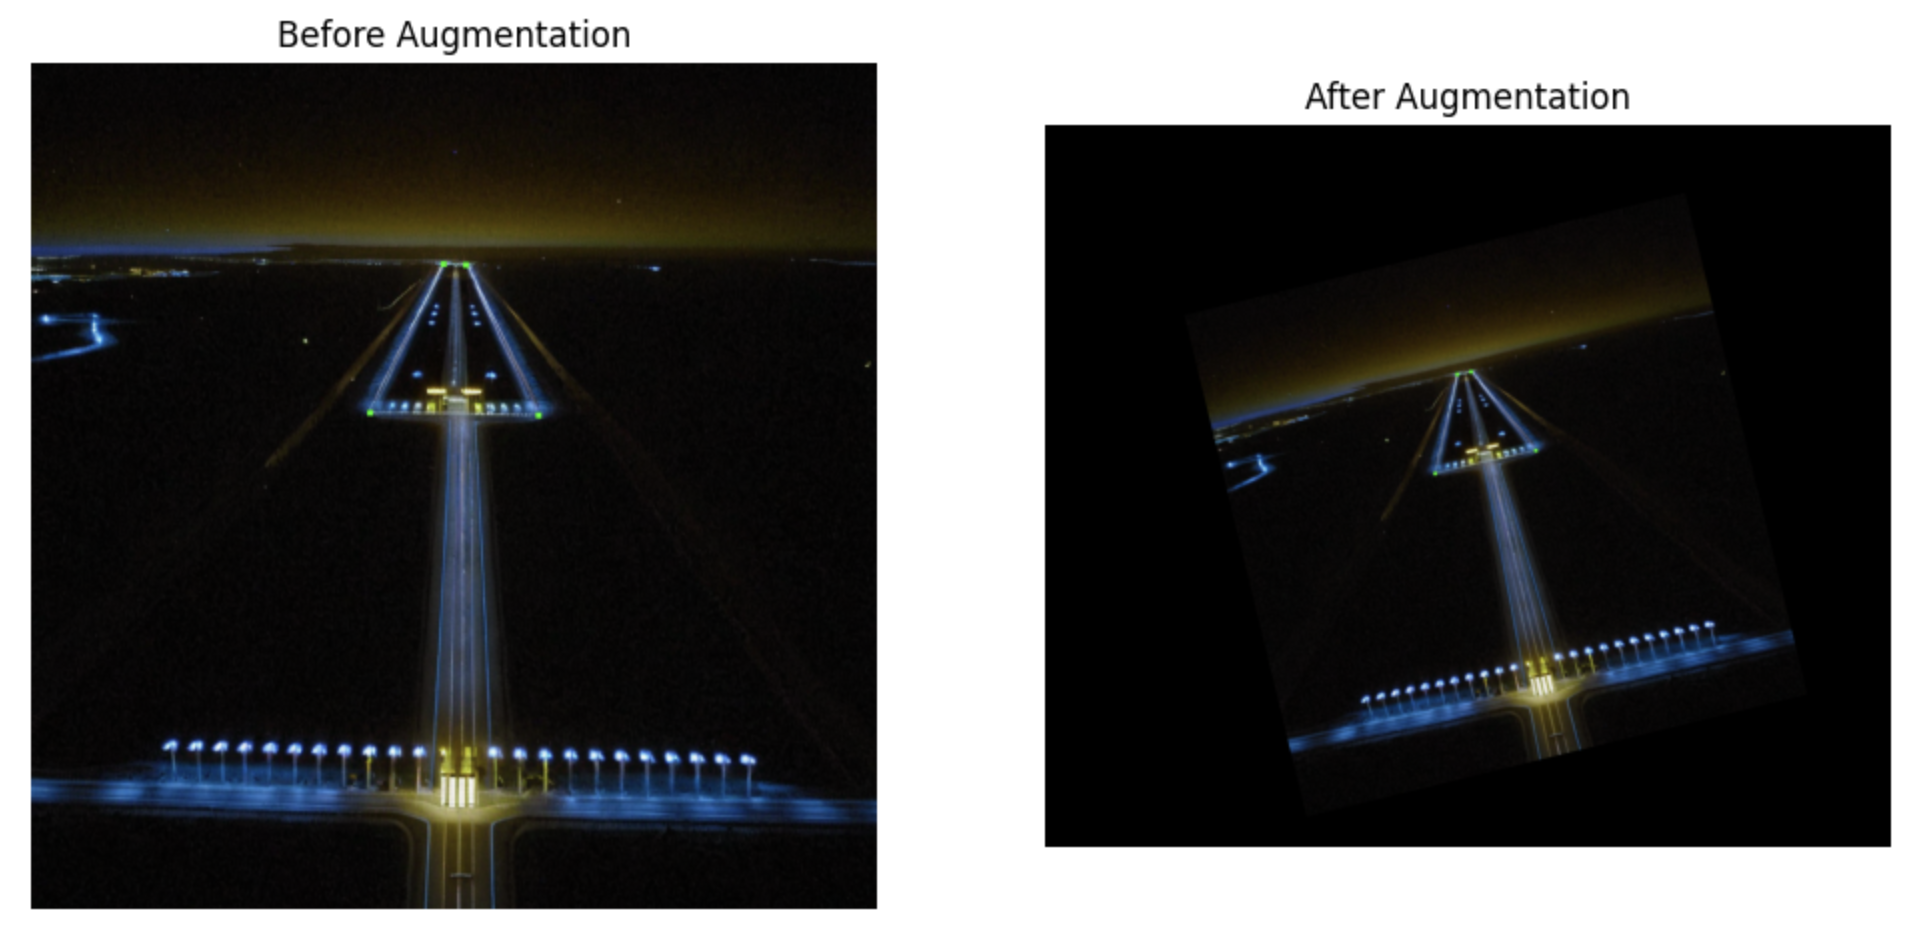
\includegraphics[width=1.0\textwidth]{figures/albumentations.png}
  \caption{Applying the \emph{Albumentations} pipeline to an image.}
\label{fig:noise_to_image}
\end{figure}

This pipeline generates images with black borders. 
The second pipeline uses \emph{inpainting} to fill in these black borders. 
First, OpenCV-based inpainting is used, filling the black border with colors from the nearby region. 
Then, a Stable Diffusion model refines the borders for better blending.

OpenCV implements Alexandru Telea's inpainting algorithm [TODO: ADD CITATION TO
TELEA] via \texttt{cv2.inpaint} with the \texttt{cv2.INPAINT\_TELEA} flag:

\begin{lstlisting}
mask = np.all(image == 0, axis=2).astype(np.uint8) * 255
kernel = np.ones((3, 3), np.uint8)
mask = cv2.dilate(mask, kernel, iterations=4)
image = Image.fromarray(cv2.cvtColor(
    cv2.inpaint(image, mask, 3, cv2.INPAINT_TELEA),
    cv2.COLOR_BGR2RGB
))
\end{lstlisting}

After this initial inpainting, a Stable Diffusion XL Inpainting pipeline is used to process the image. 
The original prompts used for the base images are reused, along with a blurred mask for smoother blending:

\begin{lstlisting}
pipe = StableDiffusionXLInpaintPipeline.from_pretrained(
    "lykon/dreamshaper-xl-lightning",
    torch_dtype=torch.float16,
    variant="fp16",
).to("cuda")
pipe.scheduler = DPMSolverMultistepScheduler.from_config(pipe.scheduler.config)

# [...]

mask = pipe.mask_processor.blur(Image.fromarray(mask), blur_factor=75)

result = pipe(
    prompt=data["prompt"],
    negative_prompt=data["negative_prompt"],
    image=image,
    mask_image=mask,
    strength=0.8,
    generator=generator,
    num_inference_steps=30,
    guidance_scale=2,
).images[0]
\end{lstlisting}

The third pipeline reads the images output by the second pipeline and creates a new folder with the same images, further augmented with weather occlusion effects done by \texttt{imgaug} \cite{???}. 
Effects are chosen depending on the variant:

\begin{itemize}
\item Clouds for \emph{pure} \texttt{day/night/dusk/dawn} images
\item Fog for \texttt{fog} images
\item Rain for \texttt{rain} images
\item Snowflakes for \texttt{snow} images
\end{itemize}

For example:

\begin{lstlisting}
if variant in ["day", "night", "dusk", "dawn"]:
    aug = iaa.SomeOf((1, 2), [
        iaa.CloudLayer(...),
        iaa.CloudLayer(...),
    ])
    image = aug(image=image)
    applied_effects.append("clouds")
elif variant in ["fog", "fog+night"]:
    aug = iaa.CloudLayer(...)
    image = aug(image=image)
    applied_effects.append("fog")
elif variant in ["rain", "rain+night"]:
    aug = iaa.Rain(drop_size=(0.1, 0.2), speed=(0.01, 0.05))
    image = aug(image=image)
    applied_effects.append("light_rain")
elif variant in ["snow", "snow+night"]:
    aug = iaa.Snowflakes(flake_size=(0.1, 0.3), speed=(0.01, 0.05))
    image = aug(image=image)
    applied_effects.append("snowflakes")
\end{lstlisting}

After each augmentation pipeline, the label JSON file is enriched with data to ensure reproducibility, including random seeds and applied transformations.

\section{Filtering Tool}

A manual filtering tool was implemented in Python with OpenCV to assist in selecting template images. 
It reads images from a directory and allows pressing \texttt{Space} to select an image or \texttt{X} to discard. 
Selected images are copied into a new directory, and a log file retains progress so the tool can be closed and resumed later without starting from scratch.

Due to time constraints, template images were filtered as follows:
\begin{enumerate}
\item Use all images from \texttt{LARD\_test\_real\_nominal} as template images, pass them through the canny-edge and base-image generation modules, generating one daylight base image per template.
\item Use the filtering tool to select which base images had easily recognizable runways with consistent markings and structure.
\item In the end, 361 images were selected, and only these canny edges were used to generate all images in the final dataset.
\end{enumerate}

\section{The final datasets}

Three datasets are published:

\begin{enumerate}
\item \texttt{BaseImages}: containing 6498 images (18 variations for each of the 361 canny edge images).
\item \texttt{VariantImages}: containing 19494 images (3 variations for each base image) \emph{before} weather occlusion.
\item \texttt{VariantImagesWithOcclusion}: also 19494 images, same as \texttt{VariantImages} but with weather effects applied.
\end{enumerate}

Each image is associated with four files:
\begin{enumerate}
\item \texttt{.png} file (the image itself).
\item \texttt{.json} file (the image label).
\item \texttt{.mask.png} file (a segmentation mask: black background, white runway).
\item \texttt{.txt} file (a YOLO-format label for detection/segmentation training).
\end{enumerate}

The JSON label file carries the runway keypoints as well as all data required for reproducing that specific image, including prompts, seeds, variant details, transformations, and so on. 
This metadata supports image classification (by variant or weather type), label fixes without regenerating images, and easier reproducibility/peer review.

Each directory also includes \texttt{train.txt}, \texttt{test.txt}, and \texttt{val.txt} splits in 80/10/10 proportions, ensuring images sharing the same source canny edge (and thus similar structure) do not leak from training into testing.

\section{Generated images}


To demonstrate a sample of generated images, three random template images were
chosen. Two are close-up shots and the third is a far away picture. They
are shown as three grids of images of for rows.

The first row contains the template image, the canny edge extracted from it,
and the runway label mask. The second row contains three images from the Base
Images dataset generated from the template image. The third row contains three
images from the Variant Images dataset, generated from the Base Images. The
fourth row contains three images from the Variant Images with Occlusion dataset,
associated with the shown Variant Images.

\begin{figure}[htbp]
\centering
\includegraphics[width=1.2\textwidth]{figures/GeneratedImage1.png}
  \caption{Template image \emph{"9xG0a8TUdXg\_028"} }
\label{fig:noise_to_image}
\end{figure}

\begin{figure}[htbp]
\centering
\includegraphics[width=1.2\textwidth]{figures/GeneratedImage2.png}
  \caption{Template image \emph{"0CLSYZPFbTg\_110"} }
\label{fig:noise_to_image}
\end{figure}

\begin{figure}[htbp]
\centering
\includegraphics[width=1.2\textwidth]{figures/GeneratedImage3.png}
  \caption{Template image \emph{"0P-HJgLkZLk\_085"} }
\label{fig:noise_to_image}
\end{figure}
